\chapter{Entwickler Dokumentation}
\label{entw_docu}
In dem folgenden Kapitel wird die Einrichtung, zur Benutzung der CIRS-APP, beschrieben. Dabei werden sowohl die notwendigen Software Tools genannt, als auch die Nutzung zum starten der APP auf einem Android Emulator und einem Android Smartphone.

\section{Voraussetzungen}
\label{voraussertungen}
Für die Nutzung der App wird ein Backend Server benötigt. Um die Server Software auszuführen benötigen Sie:
\begin{itemize}
\item Node.js, hier zu finden \url{https://nodejs.org/en/} (die LTS Version ist zu bevorzugen)
\item Git
\end{itemize}
Für die Kompelierung der App benötigen Sie die folgenden Software-Tools:
\begin{itemize}
\item Flutter SDK, hier zu finden \url{https://flutter.dev/docs/get-started/install}
\item Git
\item JDK 8, hier zu finden \url{https://www.oracle.com/de/java/technologies/javase/javase-jdk8-downloads.html}
\item Android Studio, dies kann zusammen mit dem Android Studio heruntergeladen werden \url{https://developer.android.com/studio}
\item 
\end{itemize}
Laden Sie die Backend Server Software vom Github-Repository \url{https://github.com/amandajoelle/Backend} herunter. Sie können diese als Zip-Datei herunterladen oder mit dem Befehl \textit{git clone https://github.com/amandajoelle/Backend.git}.\\
Laden Sie sich anschließend die CIRS-APP herunter, vom Github-Repository \url{https://github.com/amandajoelle/Frontend}.

\section{Benutzung}
\label{benutzung}
Zuerst müssen die benötigten Abhängigkeiten heruntergeladen werden, hierfür muss der Befehl \textit{npm install} im Ordner Backend ausgeführt werden. Erstellen Sie im Backend-Ordner eine \textit{.env} Datei. Diese sollte mit Umgebungsvariablen initialisiert werden. Dies können Sie der README.md entnehmen.\\
Anschließend muss die Datenbank erstellt werden. Mithilfe des Befehles \textit{npm run database} wird eine Datenbank im Unterordner \textit{database} erstellt. Hier befindet sich nun die Datei \textit{cirs.db}, welche alle Datenbankeinträge beinhaltet. Abschließend muss die Backend Server Software nur noch mit dem Kommando \textit{npm run dev} gestartet werden.
\\[0.5cm]
Für die Kompilierung und Nutzung der CIRS-APP in einem Android Emulator, installieren Sie Android Studio und fügen Sie dem AVD einen Emulator hinzu.
\begin{figure}[hbt!]
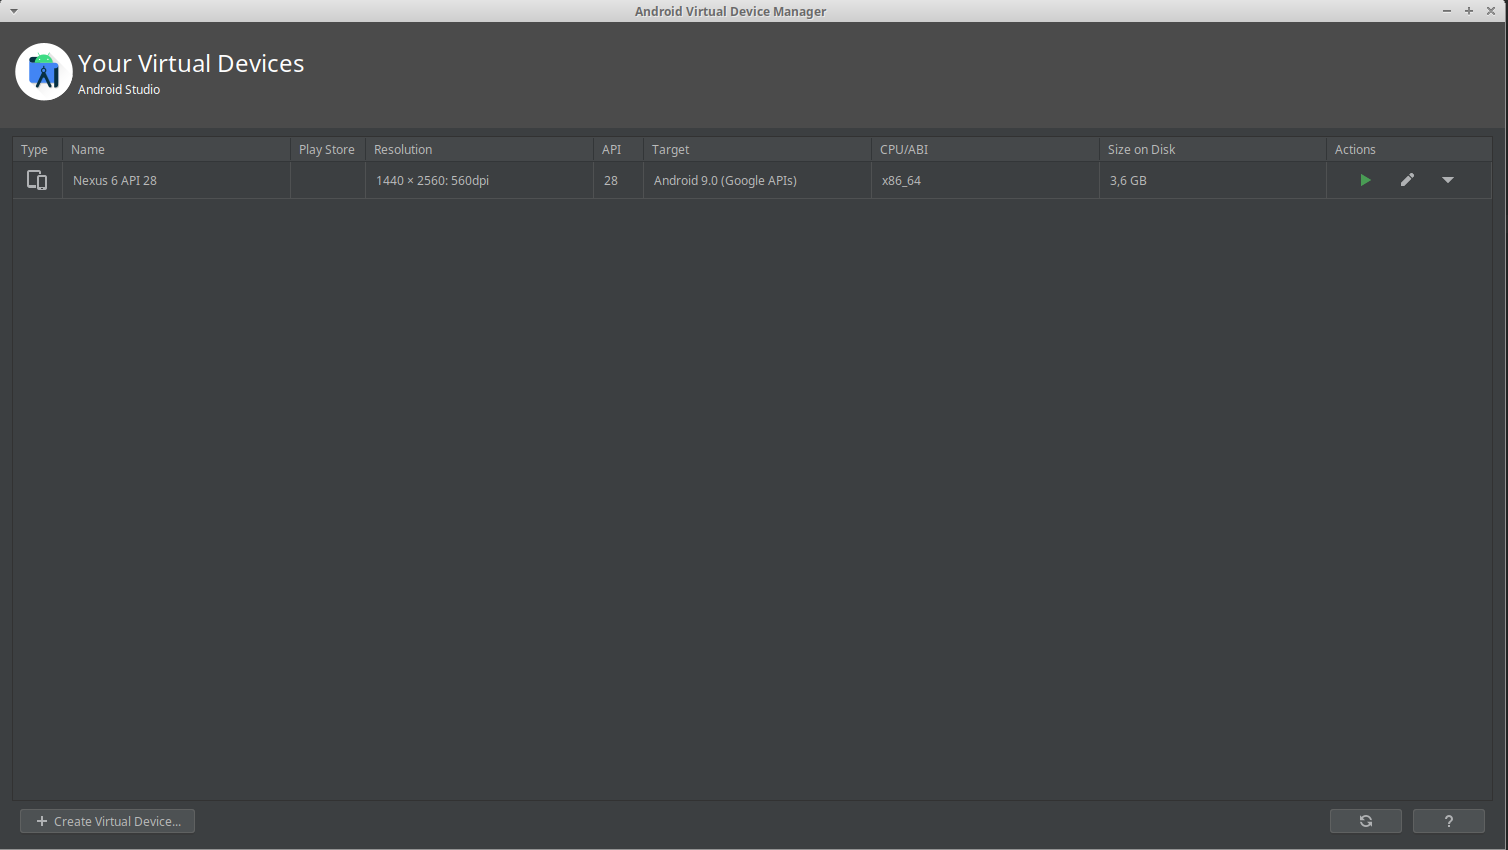
\includegraphics[width=16cm]{AVD.png}
\caption{AVD Menü zum erstellen und starten von Android Emulatoren}
\label{fig:avd}
\end{figure}
Starten Sie den Android Emulator und für Sie in einem Terminal, im Frontend Ordner, den Befehl \textit{flutter run --release} aus.
\\[0.5cm]
Im Login Bildschirm der App, können Sie ich mit einem Beispiel Nutzer anmelden, um Fälle zu bearbeiten. Die Zugangsdaten sind:
\begin{itemize}
\item E-Mail: Mueller@cirs.de
\item Passwort: 123456789
\end{itemize}
Die App kann ebenfalls auf einem Android Smartphone ausgeführt werden. Hierfür muss in der Datei \textit{main.dart}, im Verzeichnis \textit{frontend/lib} die ServerUrl geändert werden.
\begin{lstlisting}[language=Java, caption=ServerUrl ersetzen, label=lst:url_ersetzen]
...
final String serverUrl = 'http://10.0.2.2:8080';

void main() {
  runApp(MyApp());
}
...
\end{lstlisting}
Ersetzen Sie die IP Adresse in der Konstanten \textit{serverUrl}, aus dem Listing \ref{lst:url_ersetzen}, für die Ihres Computers auf dem die Backend Server Software ausgeführt wird. Sowohl \textit{http://} als auch \textit{:8080} müssen Bestandteil der URL bleiben.

\section{Workflow}
\label{workflow}
Für die Benutzung der wurde ein basischer Workflow erarbeitet, der Meldung eines Vorfalles beschreibt. In der Abbildung \ref{fig:work} wird dieser Workflow dargestellt.
\begin{figure}[hbt!]
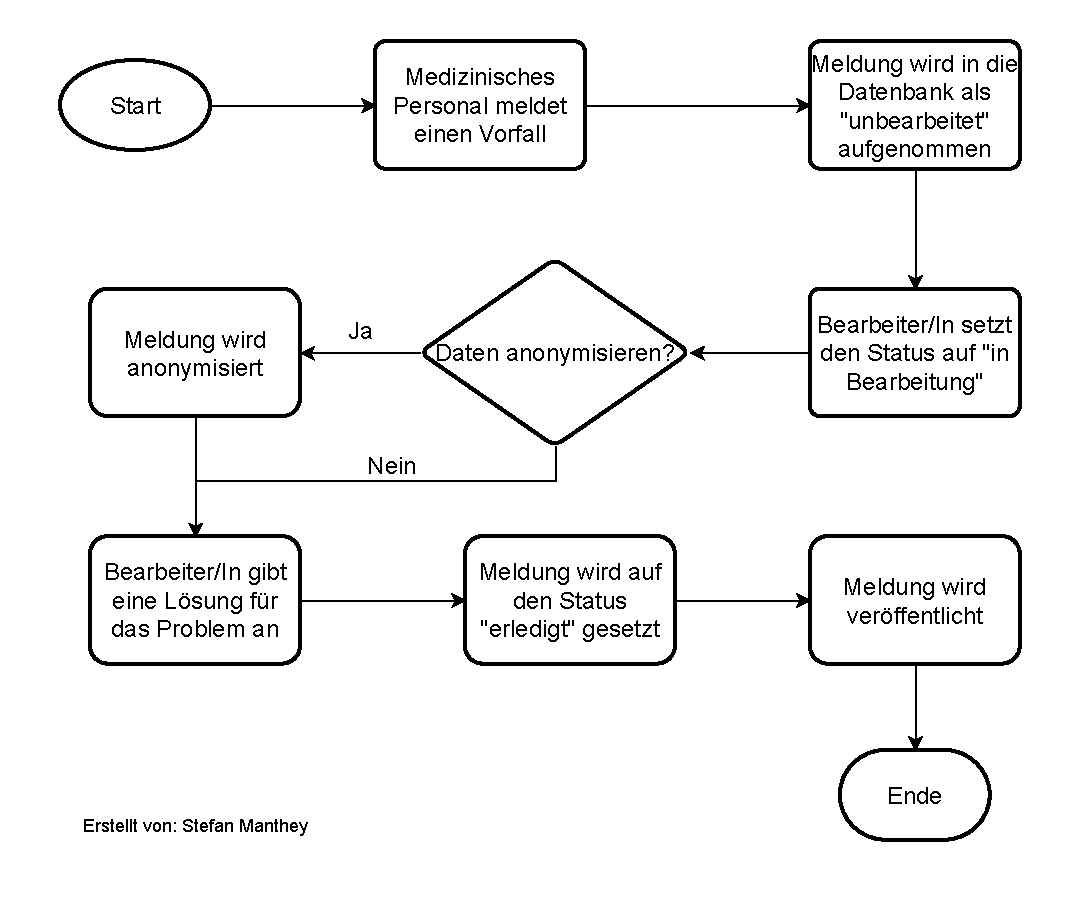
\includegraphics[width=16cm]{CIRS_Workflow.pdf}
\caption{Grundlegender Workflow zum melden eines Vorfalls in der CIRS APP}
\label{fig:work}
\end{figure}

\section{Datenbank}
\label{datenbank}
Für die Sicherung der Daten wurde eine relationale Datenbank verwendet. Im Rahmen des Projektes wurde dies mit SQLite erstellt. Diese kann später, ohne Änderungen im Programmcode, durch eine andere relationale Datenbank ersetzt werden. In der Abbilding \ref{fig:cirs_data} wird das Entity-Relationship-Modell, für die erstellte Datenbank, abgebildet.
\begin{figure}[hbt!]
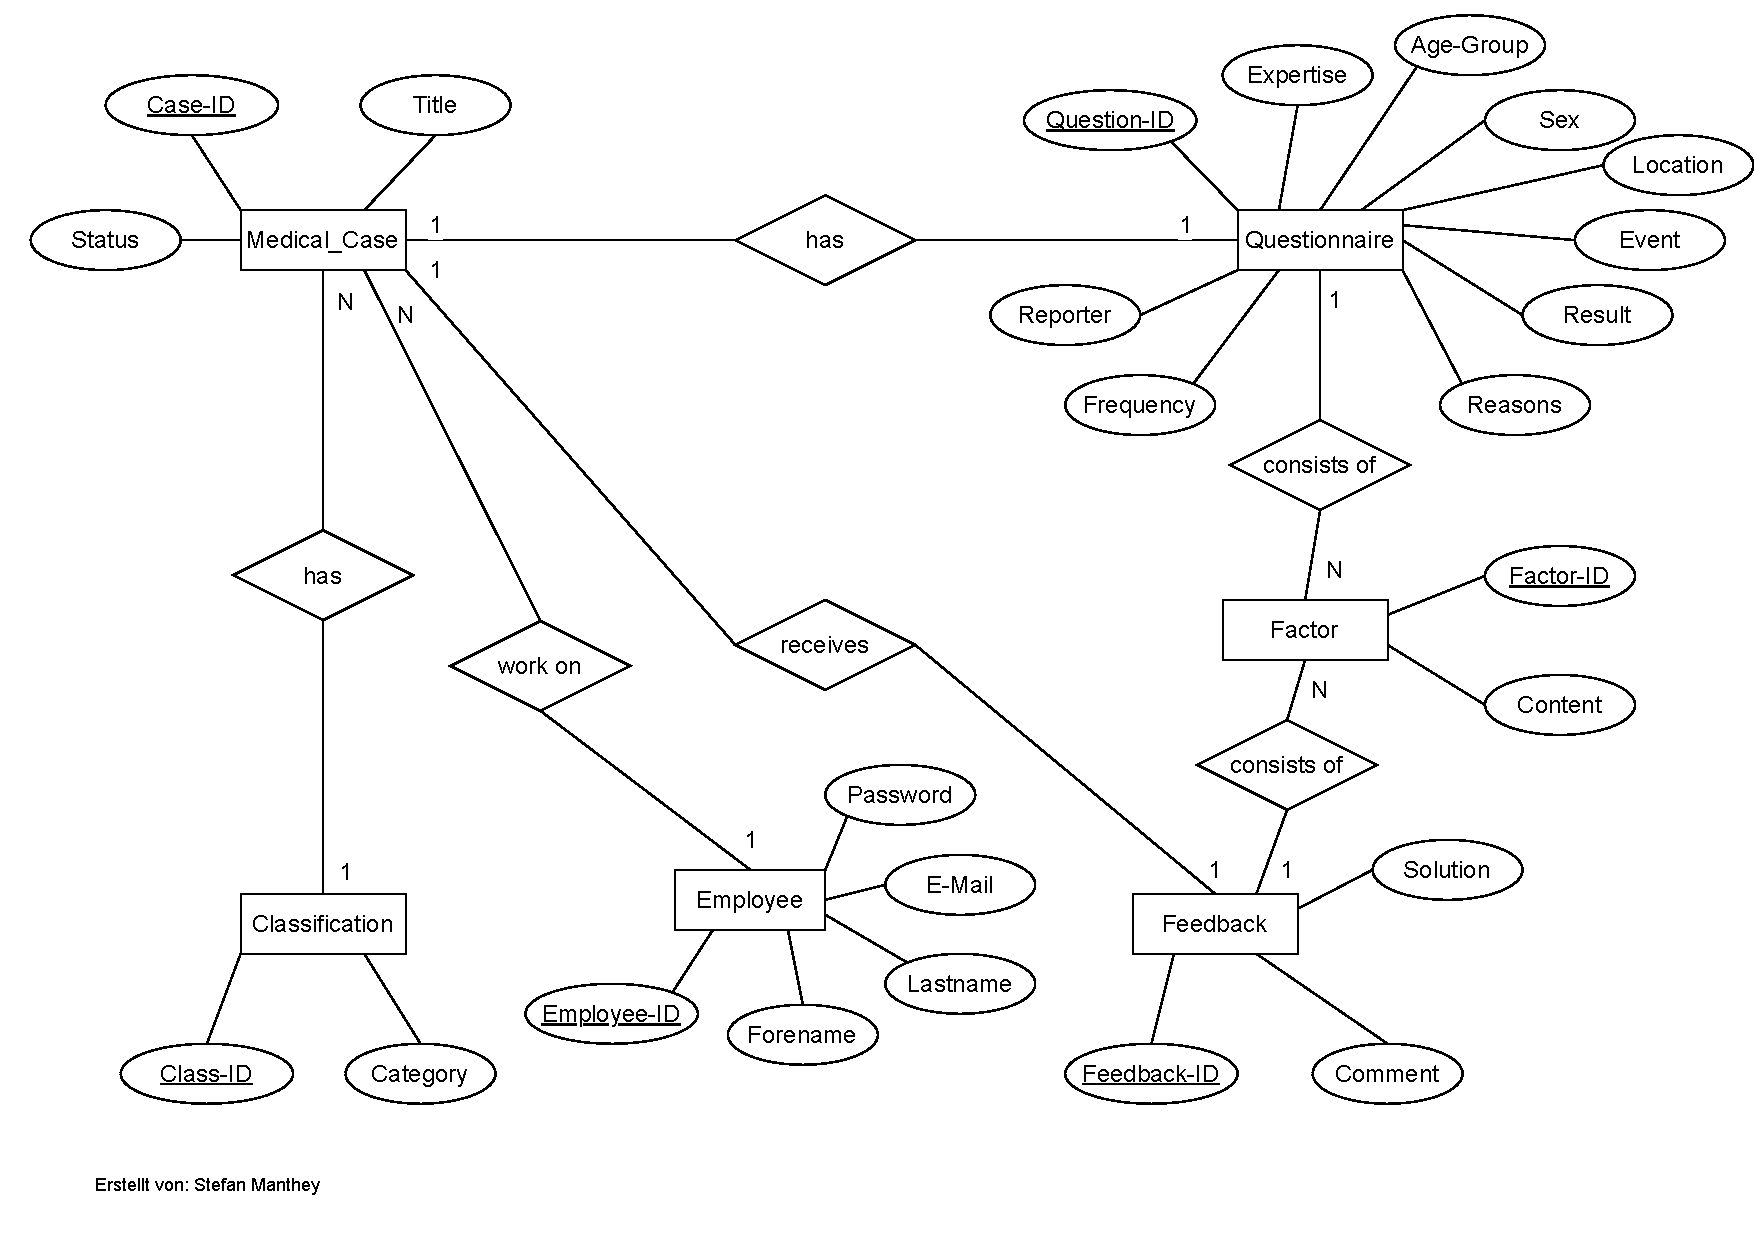
\includegraphics[width=16cm]{ERM-CIRS.pdf}
\caption{Entity-Relationship-Modell für die CIRS Datenbank}
\label{fig:cirs_data}
\end{figure}